\documentclass[12pt,a4paper]{article}

% ------------------------------------------------------------
% PACKAGES
% ------------------------------------------------------------
\usepackage[a4paper,margin=1in]{geometry}
\usepackage{graphicx}
\usepackage{float}
\usepackage{array}
\usepackage{tabularx}
\usepackage{listings}
\usepackage{xcolor}
\usepackage{setspace}
\usepackage{ragged2e}
\usepackage{titlesec}
\usepackage{enumitem}
\usepackage{caption}
\captionsetup{font=small,labelfont=bf,justification=centering}
\usepackage[colorlinks=true, urlcolor=blue, linkcolor=black]{hyperref}
\usepackage{xurl}
\usepackage{tikz}
\usepackage{eso-pic}
\usepackage{tocloft}

% ------------------------------------------------------------
% DOCUMENT FORMATTING
% ------------------------------------------------------------
\setstretch{1.15}

\setlength{\parindent}{0pt}
\setlength{\parskip}{6pt}
% ------------------------------------------------------------
% PAGE BORDER
% ------------------------------------------------------------
\AddToShipoutPictureBG{%
    \begin{tikzpicture}[remember picture,overlay]
        \draw[line width=0.8pt]
            ([xshift=1.2cm,yshift=1.2cm]current page.south west)
            rectangle
            ([xshift=-1.2cm,yshift=-1.2cm]current page.north east);
    \end{tikzpicture}%
}

\setlist[itemize]{
    leftmargin=2em,
    itemsep=3pt,
    topsep=3pt
}

% ------------------------------------------------------------
% SECTION FORMATTING
% ------------------------------------------------------------
\titleformat{\section}
    {\normalfont\Large\bfseries}
    {\thesection.}
    {0.5em}
    {}

\titleformat{\subsection}
    {\normalfont\large\bfseries}
    {\thesubsection}
    {0.5em}
    {}

% ------------------------------------------------------------
% TABLE FORMATTING
% ------------------------------------------------------------
\renewcommand{\arraystretch}{1.5}

% ------------------------------------------------------------
% CUSTOM ALGORITHM LANGUAGE
% ------------------------------------------------------------
\definecolor{algoblue}{RGB}{0,70,220}
\definecolor{algopurple}{RGB}{150,0,180}
\definecolor{algogreen}{RGB}{0,130,50}
\definecolor{algogray}{RGB}{100,100,100}

\lstdefinelanguage{Algorithm}{
    morekeywords={
        ALGORITHM,
        START,
        END,
        STEP
    },
    keywordstyle=\color{algoblue}\bfseries,
    sensitive=false,
    morecomment=[l]{-},
    commentstyle=\color{algogreen}
}

% ------------------------------------------------------------
% ALGORITHM LISTING STYLE
% ------------------------------------------------------------
\lstdefinestyle{algorithmstyle}{
    basicstyle=\ttfamily\small,
    backgroundcolor=\color{white},
    frame=single,
    rulecolor=\color{gray},
    numbers=left,
    numberstyle=\tiny\color{algogray},
    numbersep=8pt,
    breaklines=true,
    breakatwhitespace=false,
    keepspaces=true,
    showspaces=false,
    showstringspaces=false,
    showtabs=false,
    columns=fullflexible,
    tabsize=4,
    xleftmargin=10pt,
    framexleftmargin=10pt
}


% ------------------------------------------------------------
% TABLE OF CONTENTS FORMATTING
% ------------------------------------------------------------
\renewcommand{\contentsname}{TABLE OF CONTENTS}
\setcounter{tocdepth}{2}
\setlength{\cftbeforesecskip}{4pt}

% ------------------------------------------------------------
% DOCUMENT START
% ------------------------------------------------------------

\begin{document}
\pagenumbering{gobble}   % no page numbers on front matter
% ============================================================
% TITLE PAGE
% ============================================================

\begin{center}
\vspace{1cm}
{\large\bfseries SMART HOME WATER TANK MONITORING}\\
{\large\bfseries AND AUTOMATIC CONTROL SYSTEM}\\
{\large\bfseries WITH STATISTICAL ANALYSIS}

\vspace{0.5cm}
{\itshape As per the 4th Semester Mini Project(Embedded System)}

\vspace{0.6cm}
\textbf{Bachelor of Technology\\
Department of Electrical Engineering}

\vspace{0.6cm}
\textbf{Rupak Chatterjee} \\
Roll no.120016244041\\
\textbf{Aranyak Das} \\Roll no.120016244010\\
\textbf{Pinaki Das} \\Roll no.120016244034\\
\textbf{Pratistha Bhadra}\\ Roll no.120016244035\\
\textbf{Pritam Mondal} \\Roll no.120016244036

\vspace{0.8cm}
Under the Supervision of\\
\textbf{Kingsuk Majumdar, Ph.D.(Engg)}\\
Assistant Professor\\
Dept. of Electrical Engineering\\
BCREC, Durgapur

\vspace{2.5cm}
{\bfseries DR. B. C. ROY ENGINEERING COLLEGE}\\
{\small (An Autonomous Institute, Affiliated to MAKAUT)}\\
{\small Department of Electrical Engineering}\\
{\small Durgapur -- 713206, West Bengal, India}
\vfill
10 September 2026
\end{center}
\newpage



\pagenumbering{roman}
\setcounter{page}{1}

% PREFACE
% ============================================================
\section*{PREFACE}
\addcontentsline{toc}{section}{PREFACE}

This report presents the design and implementation of the project entitled \textbf{SMART HOME WATER TANK MONITORING AND AUTOMATIC CONTROL SYSTEM WITH STATISTICAL ANALYSIS}.

The project was carried out as a Fourth Semester Mini Project in the Department of Electrical Engineering at Dr. B. C. Roy Engineering College, Durgapur.

The developed prototype integrates Arduino UNO, HC-SR04 ultrasonic sensing, relay-based automatic pump control, LCD display, LED indicators, buzzer alerts, AUTO/MANUAL switching through a toggle switch, CSV data logging, and a Python-based industrial dashboard for real-time monitoring and statistical analysis.

This report documents the complete hardware implementation, software development, testing procedure, statistical analysis, and the final outcomes achieved during the project.

\newpage


% ============================================================
% TABLE OF CONTENTS

% ============================================================

\phantomsection
\section*{ABSTRACT}
\addcontentsline{toc}{section}{ABSTRACT}



Water scarcity and inefficient water management pose significant challenges in modern urban households, leading to resource wastage, increased electricity consumption, and damage to water pumping infrastructure. This project presents the design and development of a Smart Home Water Tank Monitoring and Automatic Control System that integrates embedded systems, sensor technology, and data analytics to provide an intelligent, low-cost solution for automated water level regulation.

The system employs an Arduino Uno microcontroller interfaced with an HC-SR04 ultrasonic sensor to continuously measure the water level in an overhead tank in real-time. Based on predefined threshold levels (ranging from empty to overflow prevention), the system automatically controls a water pump via a 1-channel relay module, ensuring the pump operates only when necessary. A 16×2 LCD display provides real-time visual feedback on water level status and system conditions, while LED indicators and a buzzer generate audio-visual alerts for critical states such as empty tank, filling, full tank, and overflow prevention. A manual override feature is also incorporated for user intervention when required.

Beyond real-time automation, the system incorporates data logging and statistical analysis capabilities. Water level readings, pump ON/OFF durations, refill frequencies, and operational timestamps are recorded in CSV format. This logged data is subsequently analyzed using Python (with libraries such as Pandas, Matplotlib, and PySerial) and Microsoft Excel to generate meaningful insights, including daily/weekly consumption patterns, peak usage hours, pump efficiency metrics, and potential water wastage trends. These analytics empower users to make informed decisions regarding their water consumption habits.

The system successfully demonstrates automatic pump control, overflow prevention, dry-run protection, and real-time status indication while maintaining cost-effectiveness through readily available components. Experimental validation confirms the system's reliability in preventing water wastage, reducing manual intervention, and optimizing energy usage. The project serves as a scalable foundation for smart water management and can be further enhanced with IoT integration, remote monitoring, and multi-tank support.

\newpage

\clearpage
\section*{ACKNOWLEDGEMENT}
\addcontentsline{toc}{section}{ACKNOWLEDGEMENT}

We would like to express our sincere gratitude to everyone who supported and guided us throughout the successful completion of this Mini Project, \textbf{``Smart Home Water Tank Monitoring and Automatic Control System with Statistical Analysis.''}

We are deeply thankful to our project supervisor, \textbf{Kingsuk Majumdar, Ph.D.(Engg)}, Assistant Professor, Department of Electrical Engineering, for his invaluable guidance, continuous encouragement, and constructive suggestions at every stage of this project. His technical insights and constant support were instrumental in helping us overcome challenges and complete the project successfully.

We also extend our heartfelt thanks to \textbf{Prof.\ (Dr.) Shibendu Mahata}, Associate Professor \& Head of the Department of Electrical Engineering, for his encouragement and for providing the necessary departmental facilities and resources required to carry out this project.

We are grateful to all the faculty members and laboratory staff of the Department of Electrical Engineering for their cooperation and for providing access to the tools, components, and laboratory infrastructure that made this project possible.

We would also like to acknowledge the collective effort, dedication, and teamwork of our project group members --- \textbf{Rupak Chatterjee, Aranyak Das, Pinaki Das, Pratistha Bhadra, and Pritam Mondal} --- whose combined contributions in hardware design, software development, testing, and documentation brought this project to fruition.

Finally, we express our gratitude to our families and friends for their unwavering support, patience, and motivation throughout the duration of this project.
\newpage

\tableofcontents

\newpage
\listoffigures


\listoftables


\newpage
% ============================================================
% INTRODUCTION
% ============================================================

\newpage
\pagenumbering{arabic}
\setcounter{page}{1}

\section{INTRODUCTION}

Urban and residential water distribution systems in modern smart homes demand precise automation and analytical oversight to prevent resource depletion and physical infrastructure degradation. Traditional water tank systems suffer from continuous human oversight errors, leading to severe tank overflows, dry-running of motor pumps, and erratic power consumption patterns. By integrating embedded microcontroller architecture (Arduino Uno) with real-time distance telemetry and statistical data modeling, automated water level regulation systems provide a reliable, low-cost automation platform.

Thus, the project integrates:

\begin{itemize}
    \item Embedded programming
    \item Sensor interfacing
    \item Electrical control
    \item Motor/pump control
    \item Instrumentation
    \item Data logging
    \item Statistical analysis
    \item Basic home automation
\end{itemize}

% ============================================================
% REQUIREMENTS
% ============================================================

\section{REQUIREMENTS}

The project requires both hardware and software resources.

\subsection{Hardware Requirements}

\begin{itemize}
    \item Arduino Uno
    \item HC-SR04 ultrasonic sensor
    \item 16$\times$2 LCD display
    \item 1-channel relay module
    \item Buzzer
    \item LEDs
    \item Resistors
    \item Wires and connectors
    \item Breadboard
    \item Project enclosure/case
    \item Power supply and testing equipment
\end{itemize}

\subsection{Software Requirements}

\begin{itemize}
    \item Arduino IDE 2.x
    \item Python 3.13
    \item Visual Studio Code
    \item Git and GitHub
    \item Pandas
    \item Matplotlib
    \item PySerial
    \item ttkbootstrap
    \item Pillow
    \item Microsoft Excel
\end{itemize}

% ============================================================
% OBJECTIVES
% ============================================================

\section{OBJECTIVES}

The major objectives of the project are:

\subsection*{Objective 1 --- Automatic Water-Level Monitoring}

To continuously monitor the water level of a household overhead tank using an ultrasonic sensor.

\subsection*{Objective 2 --- Automatic Pump Control}

To automatically switch the pump ON or OFF according to predefined water-level conditions.

\subsection*{Objective 3 --- Overflow Prevention}

To prevent water overflow by switching OFF the pump when the tank approaches its full level.

\subsection*{Objective 4 --- Dry-Run Protection}

To incorporate protection against unnecessary pump operation under low-water or unsuitable operating conditions.

\subsection*{Objective 5 --- Real-Time Display}

To display water-level information and system status on an LCD.

\subsection*{Objective 6 --- Alert Generation}

To provide audio-visual alerts for important tank conditions using LEDs and a buzzer.

\subsection*{Objective 7 --- Data Logging}

To record water-level information, pump operating hours, refill frequency and other operational information in CSV format.

\subsection*{Objective 8 --- Statistical Analysis}

To analyze the collected data using Python and Excel to determine average consumption, peak usage periods, pump operation and water-wastage patterns.

These objectives are aligned with the design intent outlined in Section 1.

% ============================================================
% WORKING PRINCIPLE
% ============================================================

\section{WORKING PRINCIPLE AND SYSTEM OPERATION LOGIC}

The system operates based on a set of predefined threshold levels. The ultrasonic sensor continuously measures the distance from the sensor to the water surface, which is then converted into a water level percentage.

\textbf{Sensor Data Conversion:}

\begin{itemize}
    \item The distance is measured in centimeters using the time of flight of the ultrasonic pulse.
    \item Water level percentage is calculated based on the maximum and minimum possible distances (tank depth).
\end{itemize}

\textbf{System Operation Logic:}

The Arduino uses the following logic to control the pump and alerts:

% ------------------------------------------------------------
% WATER LEVEL TABLE
% ------------------------------------------------------------

\begin{table}[H]
    \centering
    \small
    \begin{tabularx}{\textwidth}{
        |>{\centering\arraybackslash}p{1.3cm}
        |>{\centering\arraybackslash}X
        |>{\centering\arraybackslash}p{2.3cm}
        |>{\centering\arraybackslash}p{2.4cm}
        |>{\centering\arraybackslash}p{2.4cm}
        |>{\centering\arraybackslash}p{3.1cm}|
    }
        \hline

        \textbf{Water Level (\%)} &
        \textbf{Condition} &
        \textbf{Pump Status} &
        \textbf{LED Indication} &
        \textbf{Buzzer Status} &
        \textbf{LCD Message} \\

        \hline

        0--10\% &
        Tank Empty &
        \textbf{ON} &
        Red LED &
        Continuous &
        ``EMPTY! PUMP ON'' \\

        \hline

        10--30\% &
        Tank Low &
        \textbf{ON} &
        Yellow LED &
        Intermittent Beep &
        ``LOW! FILLING'' \\

        \hline

        30--80\% &
        Tank Normal &
        \textbf{ON (if below 80\%) / OFF (if above 80\%)} &
        Green LED (if ON) &
        No Sound &
        ``NORMAL'' / ``PUMP ON'' \\

        \hline

        80--95\% &
        Tank Full &
        \textbf{OFF} &
        Blue LED &
        Success Beep (once) &
        ``FULL! PUMP OFF'' \\

        \hline

        $>95\%$ &
        Overflow Prevention &
        \textbf{OFF (Emergency)} &
        Red LED &
        Alarm &
        ``OVERFLOW! STOP'' \\

        \hline

    \end{tabularx}

    \caption{Water Level Monitoring and Pump Control Conditions}
    \label{tab:water_level_control}
\end{table}

% ============================================================
% ALGORITHM
% ============================================================

\section{ALGORITHM}

\subsection{Flowchart for the System Operation}

\begin{figure}[H]
    \centering
    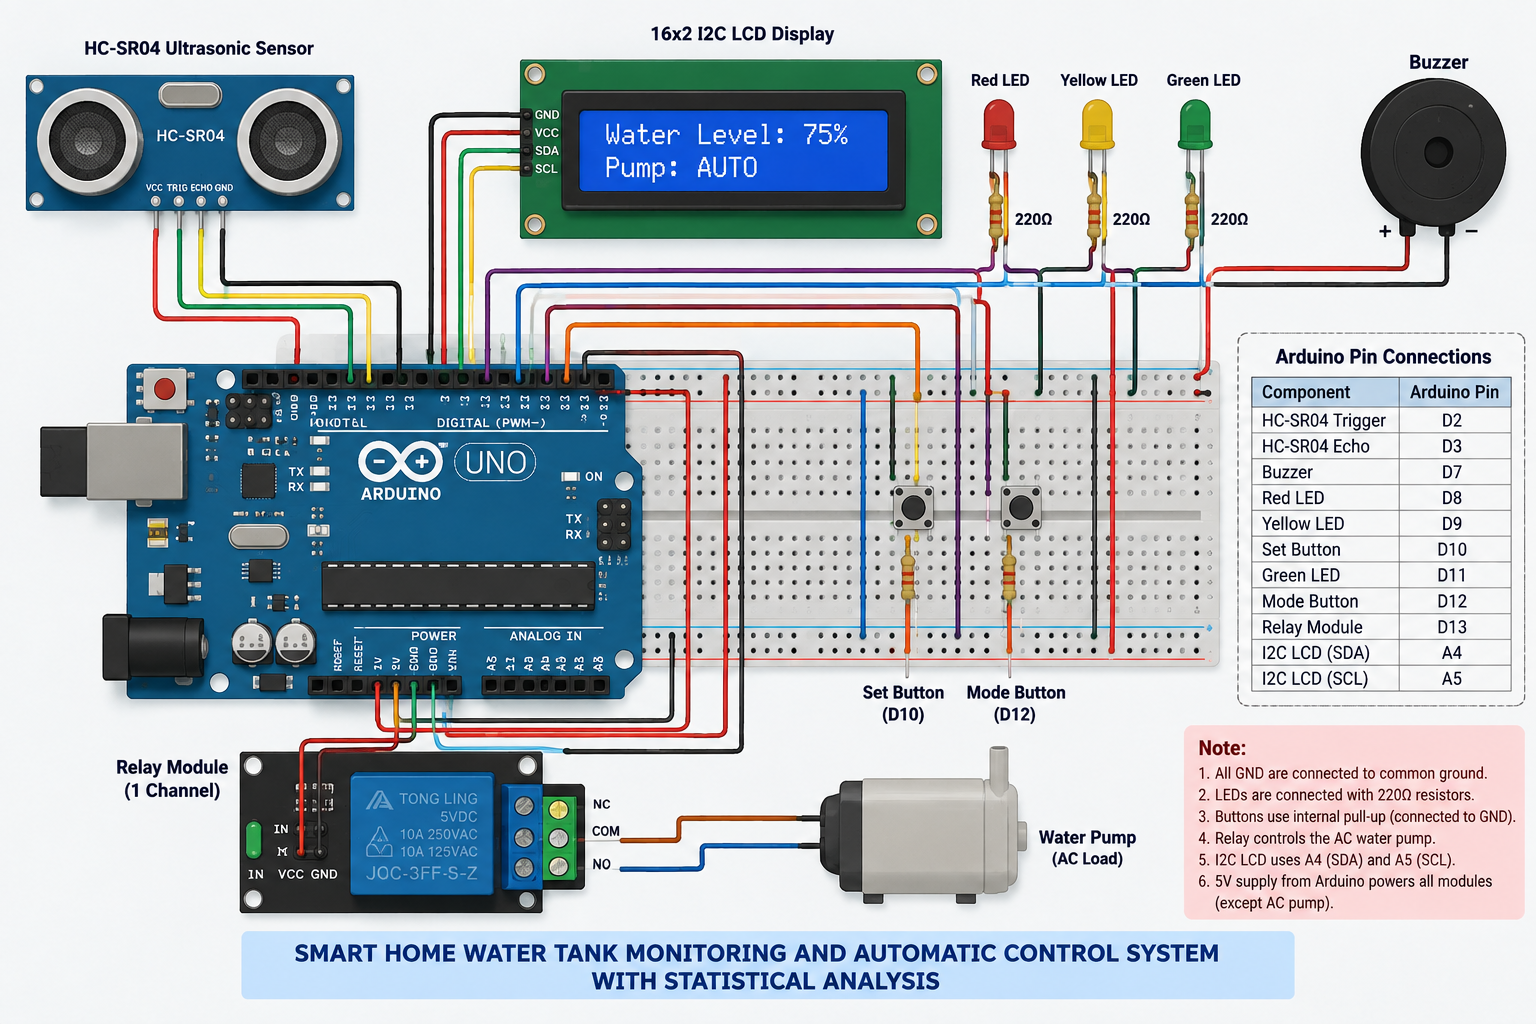
\includegraphics[width=0.82\textwidth]{../assets/circuit-diagram.png}

    \caption{System control and wiring overview}
    \label{fig:system-overview}
\end{figure}
\newpage
\textbf{ALGORITHM FOR SYSTEM OPERATION}

\lstinputlisting[
    language=Algorithm,
    style=algorithmstyle,
    caption={Algorithm for Water Level Sensing and Pump Control},
    label={lst:water-level-algorithm}
]{../Arduino_Code/Smart_Water_Tank.ino}

\section{PROJECT REPOSITORY}
\addcontentsline{toc}{section}{PROJECT REPOSITORY}

The complete source code, documentation, circuit diagrams, Python dashboard, GitHub Actions workflows, and project assets are maintained in the project's GitHub repository.

\textbf{Repository:}

\begin{figure}[H]
\centering

\includegraphics[width=0.82\textwidth]{../assets/drive_qr.png}
\caption{GitHub Repository QR Code}
\label{fig:githubqr}
\end{figure}

The repository includes:
\begin{itemize}
\item Arduino firmware
\item Python industrial dashboard
\item Circuit diagrams
\item Hardware photographs
\item Statistical analysis documentation
\item GitHub Actions validation workflows
\item Project documentation
\end{itemize}

% ============================================================
% STATISTICAL DATA ANALYSIS
% ============================================================

\subsection{Flowchart for Statistical Data Analysis}

\begin{figure}[H]
    \centering
    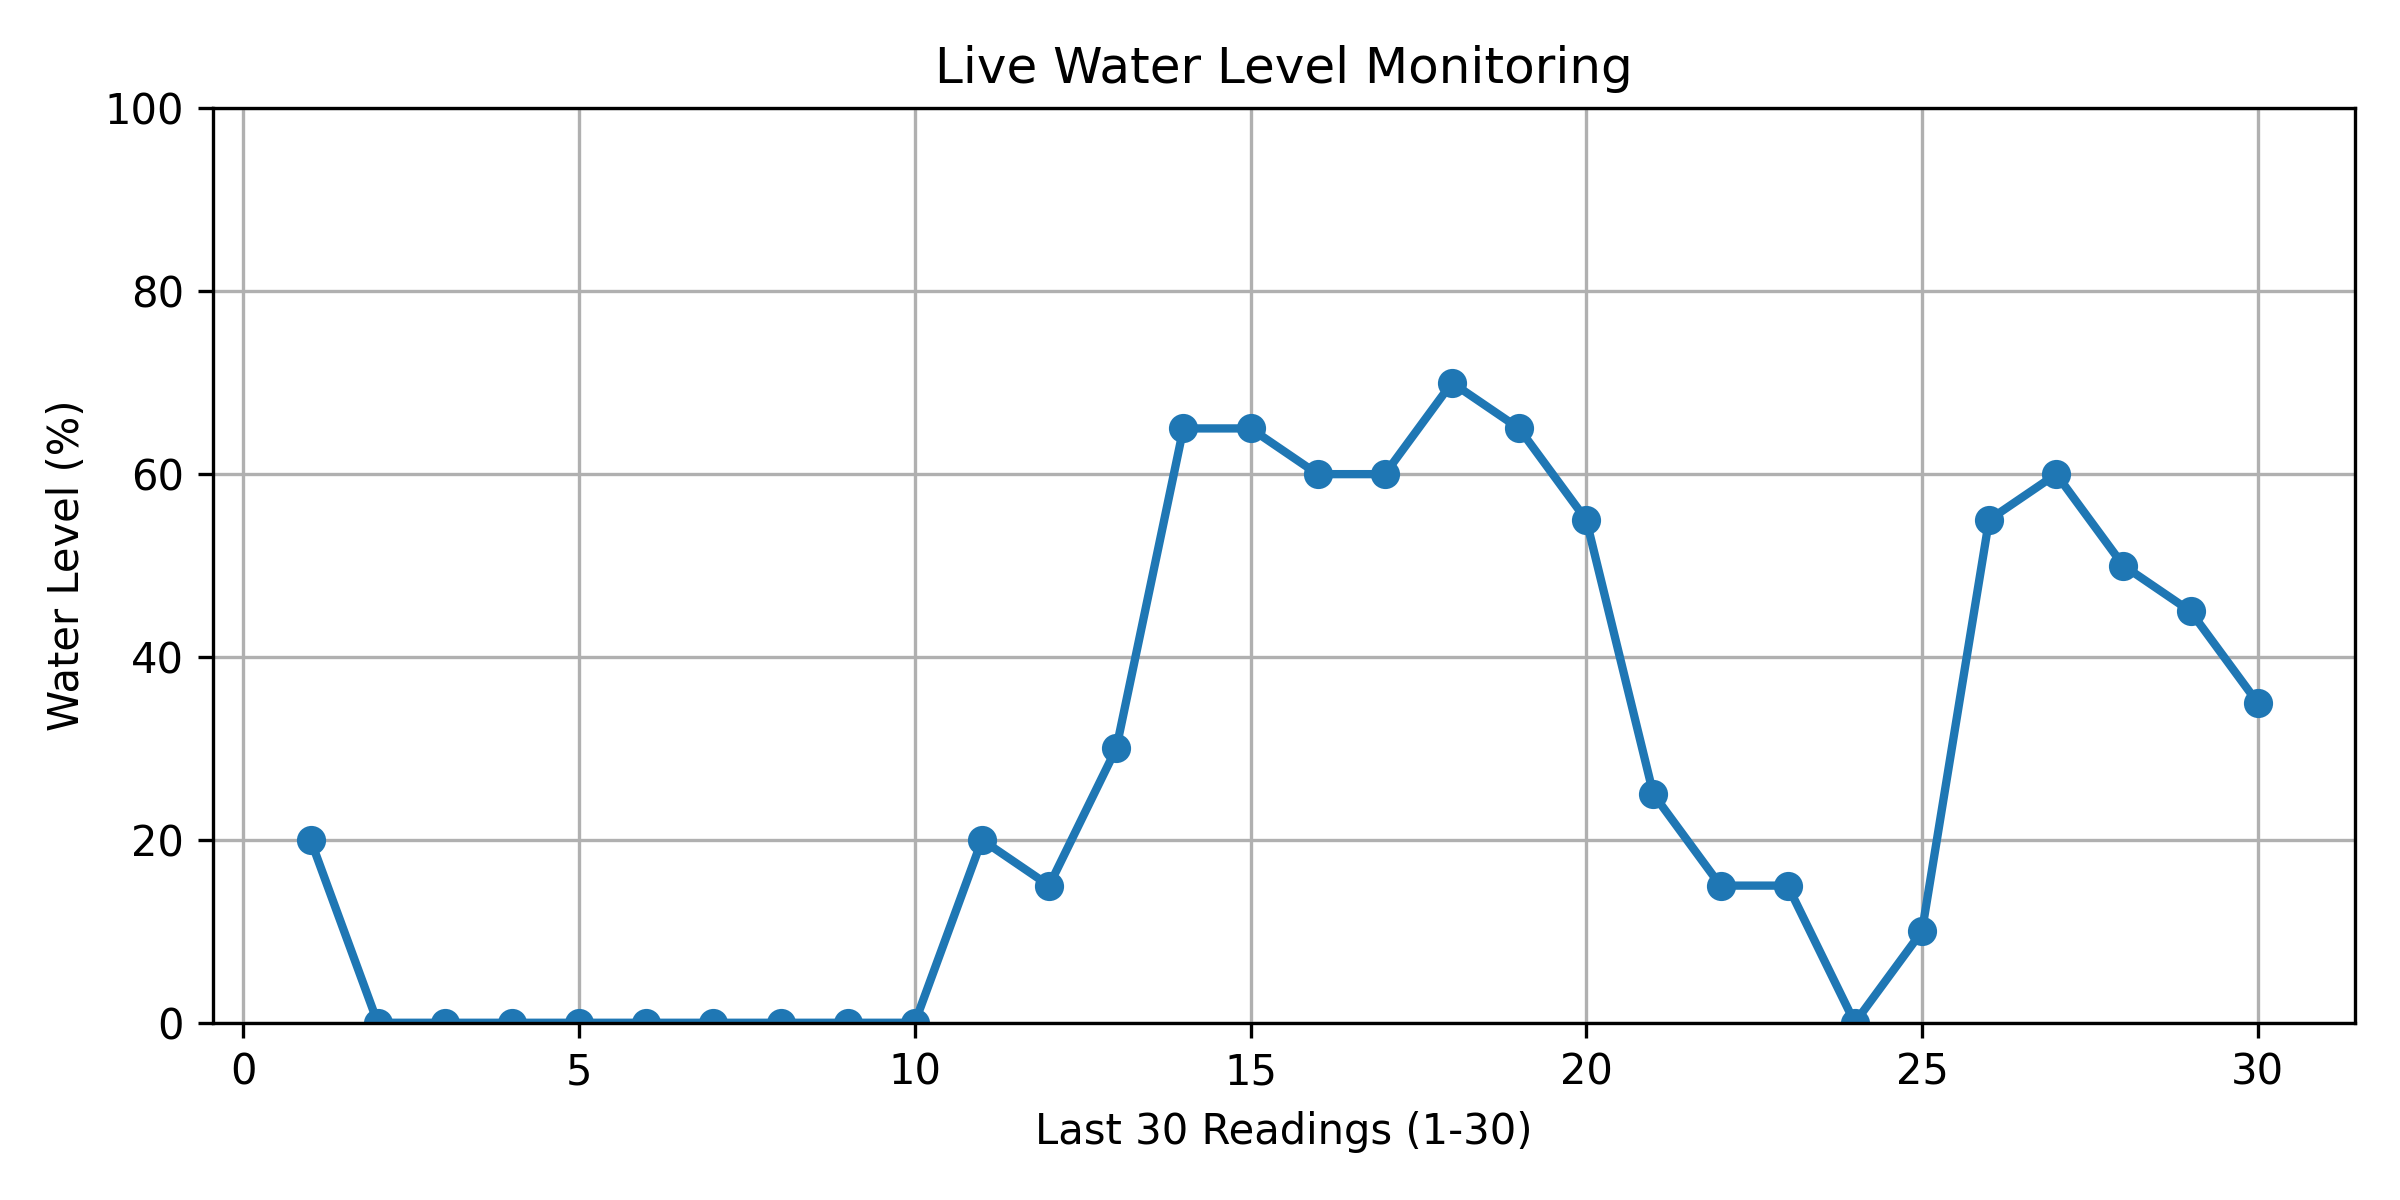
\includegraphics[width=0.82\textwidth]{../assets/water_level_graph.png}

    \caption{Water-level trend used for statistical analysis}
    \label{fig:analysis-trend}
\end{figure}


% ============================================================
% STATISTICAL ALGORITHM
% ============================================================

\textbf{Algorithm for Statistical Data Analysis}

\lstinputlisting[
    language=Algorithm,
    style=algorithmstyle,
    caption={Algorithm for Statistical Data Analysis},
    label={lst:water-consumption-algorithm}
]{../water_logger.py}

% ============================================================
% LIBRARIES
% ============================================================

\section{LIBRARIES FOR THE PROGRAM TO RUN}

\begin{itemize}
\item \textbf{pyserial} -- Reads live Arduino data through the serial port.
\item \textbf{pandas} -- Performs CSV parsing and statistical calculations.
\item \textbf{matplotlib} -- Generates live trend graphs.
\item \textbf{ttkbootstrap} -- Creates the industrial dark dashboard UI.
\item \textbf{Pillow} -- Handles dashboard icons and images.
\item \textbf{tkinter} -- Builds the desktop GUI.
\item \textbf{csv} -- Stores sensor readings in CSV format.
\item \textbf{datetime} -- Generates timestamps for every reading.
\end{itemize}

% ============================================================
% ADVANTAGES AND LIMITATIONS
% ============================================================

\section{ADVANTAGES AND LIMITATIONS}

\subsection{Advantages}

\begin{itemize}
    \item \textbf{Water Conservation:} Prevents overflow and wastage, promoting efficient water usage.

    \item \textbf{Energy Efficiency:} Automatically turns off the pump when full, saving electricity.

    \item \textbf{Convenience:} Eliminates the need for manual monitoring and pump operation.

    \item \textbf{Protection:} Prevents dry-running, which can damage the pump motor.

    \item \textbf{Data-Driven Insights:} Provides statistical analysis to help users understand and modify their consumption habits.

    \item \textbf{Cost-Effective:} Uses readily available, affordable components.
\end{itemize}

\subsection{Limitations}

\begin{itemize}
    \item \textbf{Tank Depth:} Ultrasonic sensors can be affected by tank geometry and reflections in deep or irregularly shaped tanks.

    \item \textbf{Sensitivity:} Sensor readings can be prone to errors due to dust, humidity, or temperature variations.

    \item \textbf{Single Source:} The system controls only one tank and one pump; scaling it for multi-tank or complex buildings would be more challenging.

    \item \textbf{Power Dependency:} The system relies on a stable power supply.
\end{itemize}


\section{IMPLEMENTATION AND RESULT}
The project was successfully implemented using Arduino UNO and tested under different water level conditions. The ultrasonic sensor measured the distance from the sensor to the water surface, while the Arduino calculated the corresponding water level percentage.

The LCD displayed real-time water level and pump status. The relay controlled the pump automatically according to preset thresholds. Visual indication was provided through LEDs, while the buzzer generated an alert during low-water conditions.

The Python dashboard received serial data continuously, stored readings in CSV format, and generated live graphs for statistical analysis.

\subsection{CIRCUIT DIAGRAM}

\begin{figure}[H]
    \centering
    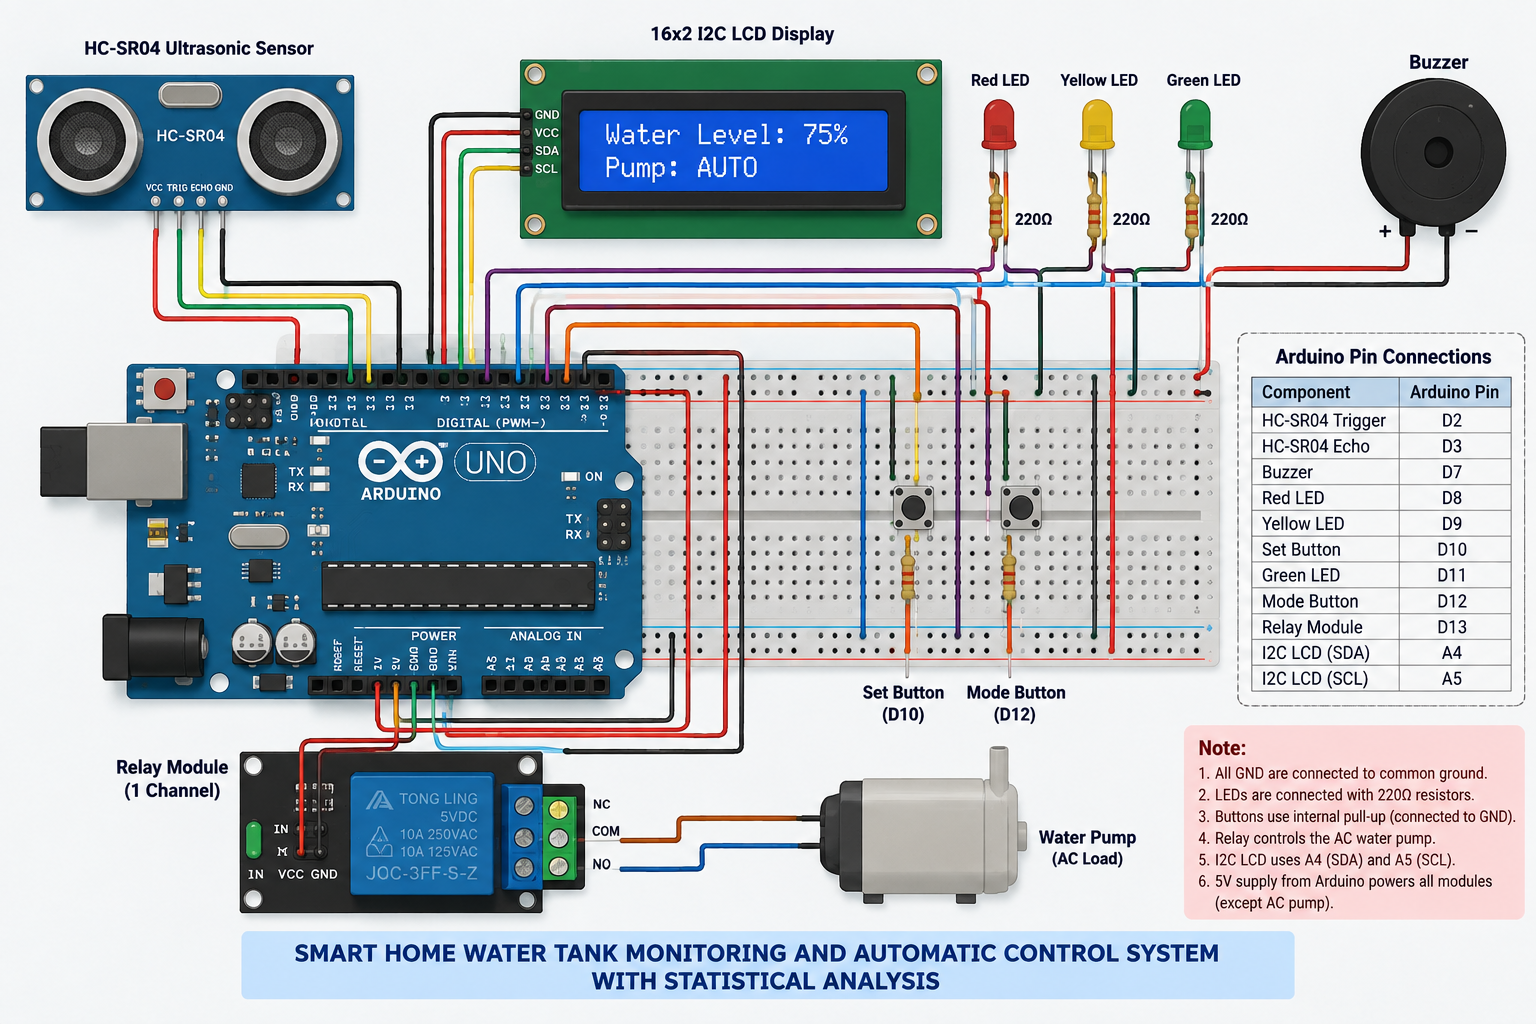
\includegraphics[width=0.82\textwidth]{../assets/circuit-diagram.png}
\caption{Circuit diagram for the Smart Water Tank}
\label{fig:circuit}
\end{figure}



\subsection{WATER LEVEL MONITORING}

\begin{figure}[H]
    \centering
    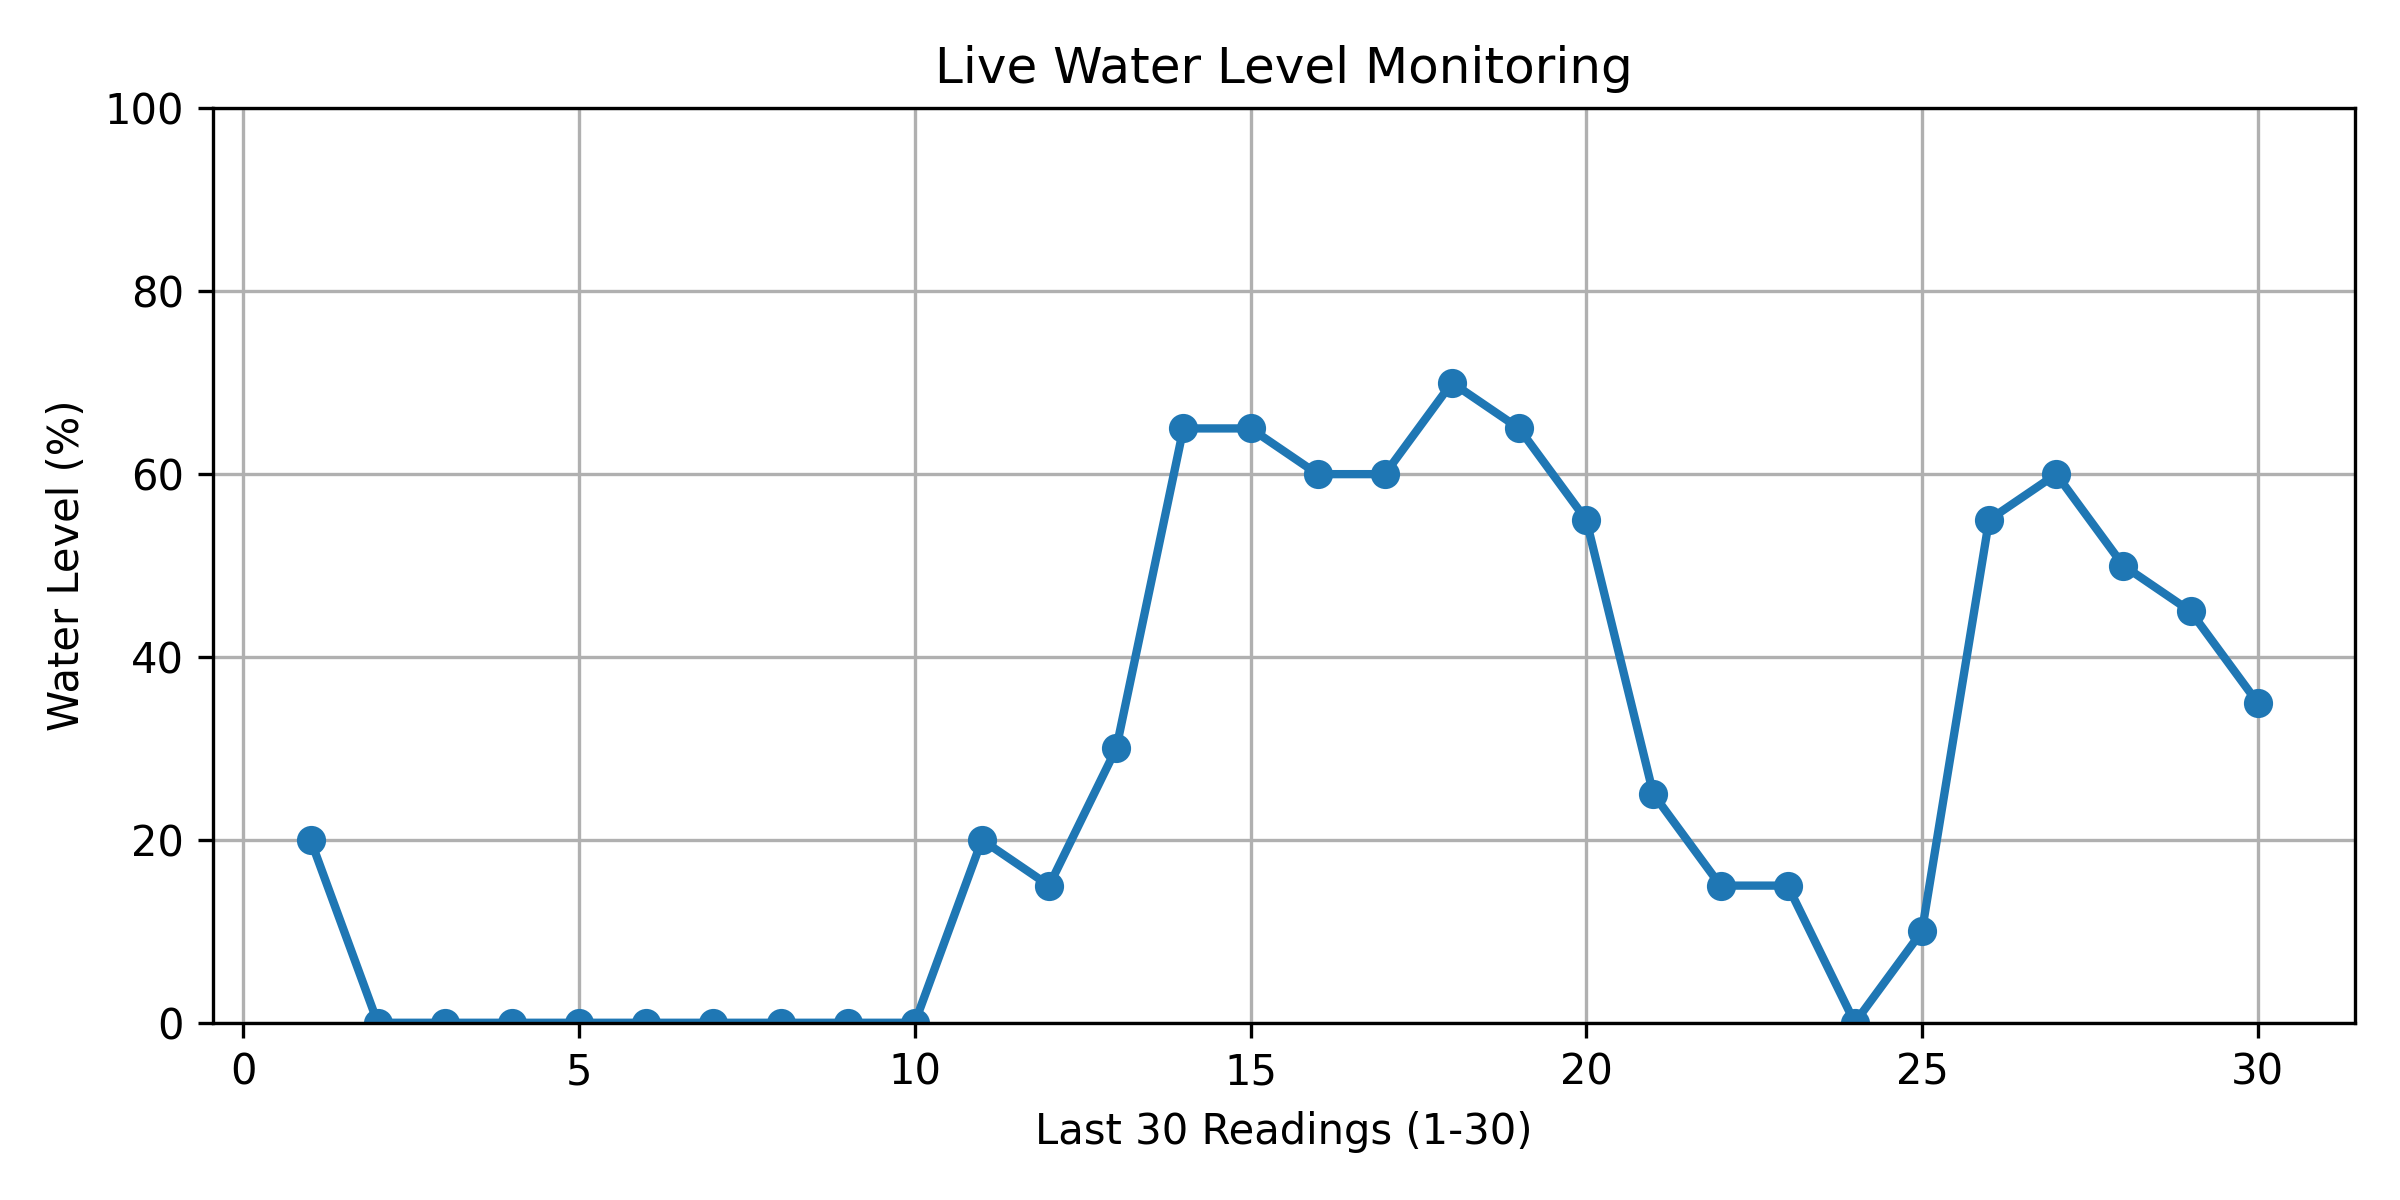
\includegraphics[width=0.82\textwidth]{../assets/water_level_graph.png}
\caption{Water level Monitoring}
\label{fig:water-level}
\end{figure}

\subsection{Python Dashboard}

\begin{figure}[H]
\centering
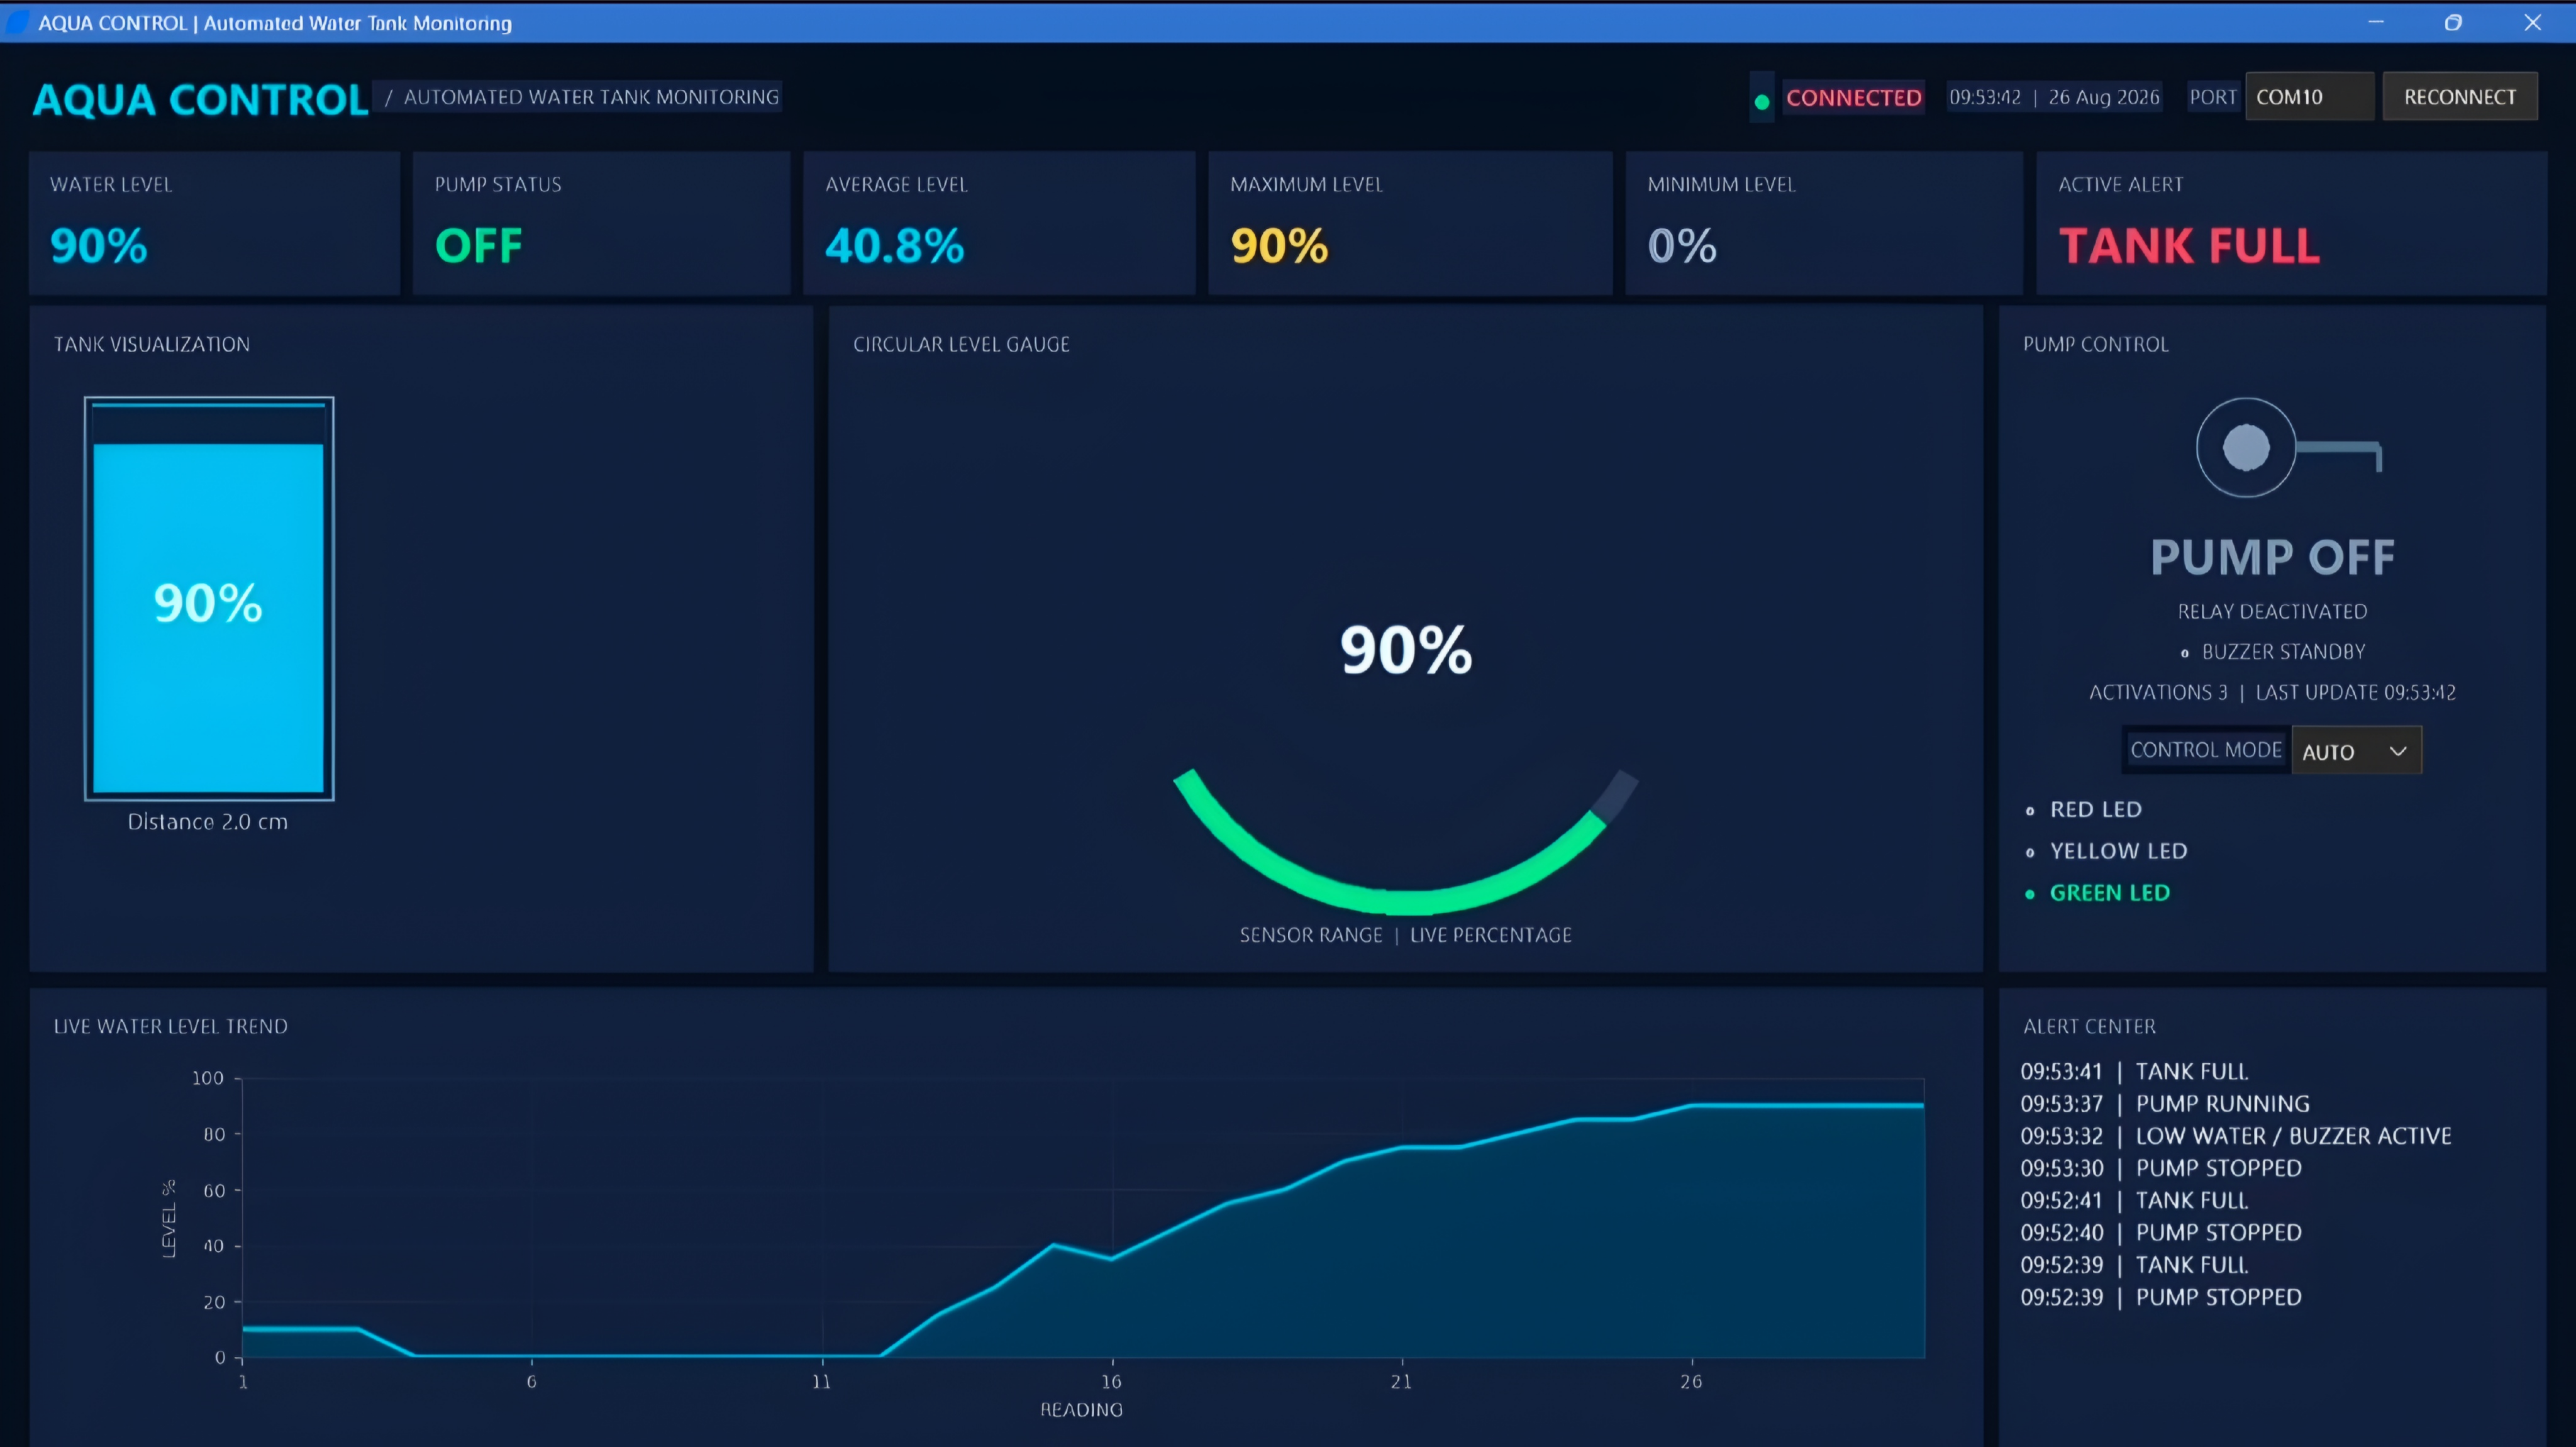
\includegraphics[width=0.82\textwidth]{../assets/dashboard-ui.png}
\caption{Industrial Python Dashboard with Live Monitoring}
\label{fig:dashboard}
\end{figure}

\textbf{Dashboard Output}

\begin{figure}[H]
\centering

\includegraphics[width=0.82\textwidth]{../assets/drive_qr.png}
\caption{Scan to view the Dashboard \& Workflow Demonstration}
\end{figure}

\subsection{Statistical Analysis Results}

The logged CSV data was analyzed using Python. The dashboard continuously calculated the average water level, maximum level, minimum level, pump activation count and live trend analysis.

\begin{itemize}
\item Average Water Level
\item Maximum Water Level
\item Minimum Water Level
\item Pump Activation Count
\item Live Trend Analysis
\end{itemize}

\begin{table}[H]
\centering
\begin{tabular}{|l|c|}
\hline
Average Level & 82.5\%\\
Maximum Level & 95\%\\
Minimum Level & 30\%\\
Pump Activations & 3\\
Current Mode & AUTO\\
\hline
\end{tabular}
\caption{Sample Statistical Output}
\label{tab:stats}
\end{table}

\subsection{HARDWARE IMPLEMENTATION}

\begin{figure}[H]
    \centering
    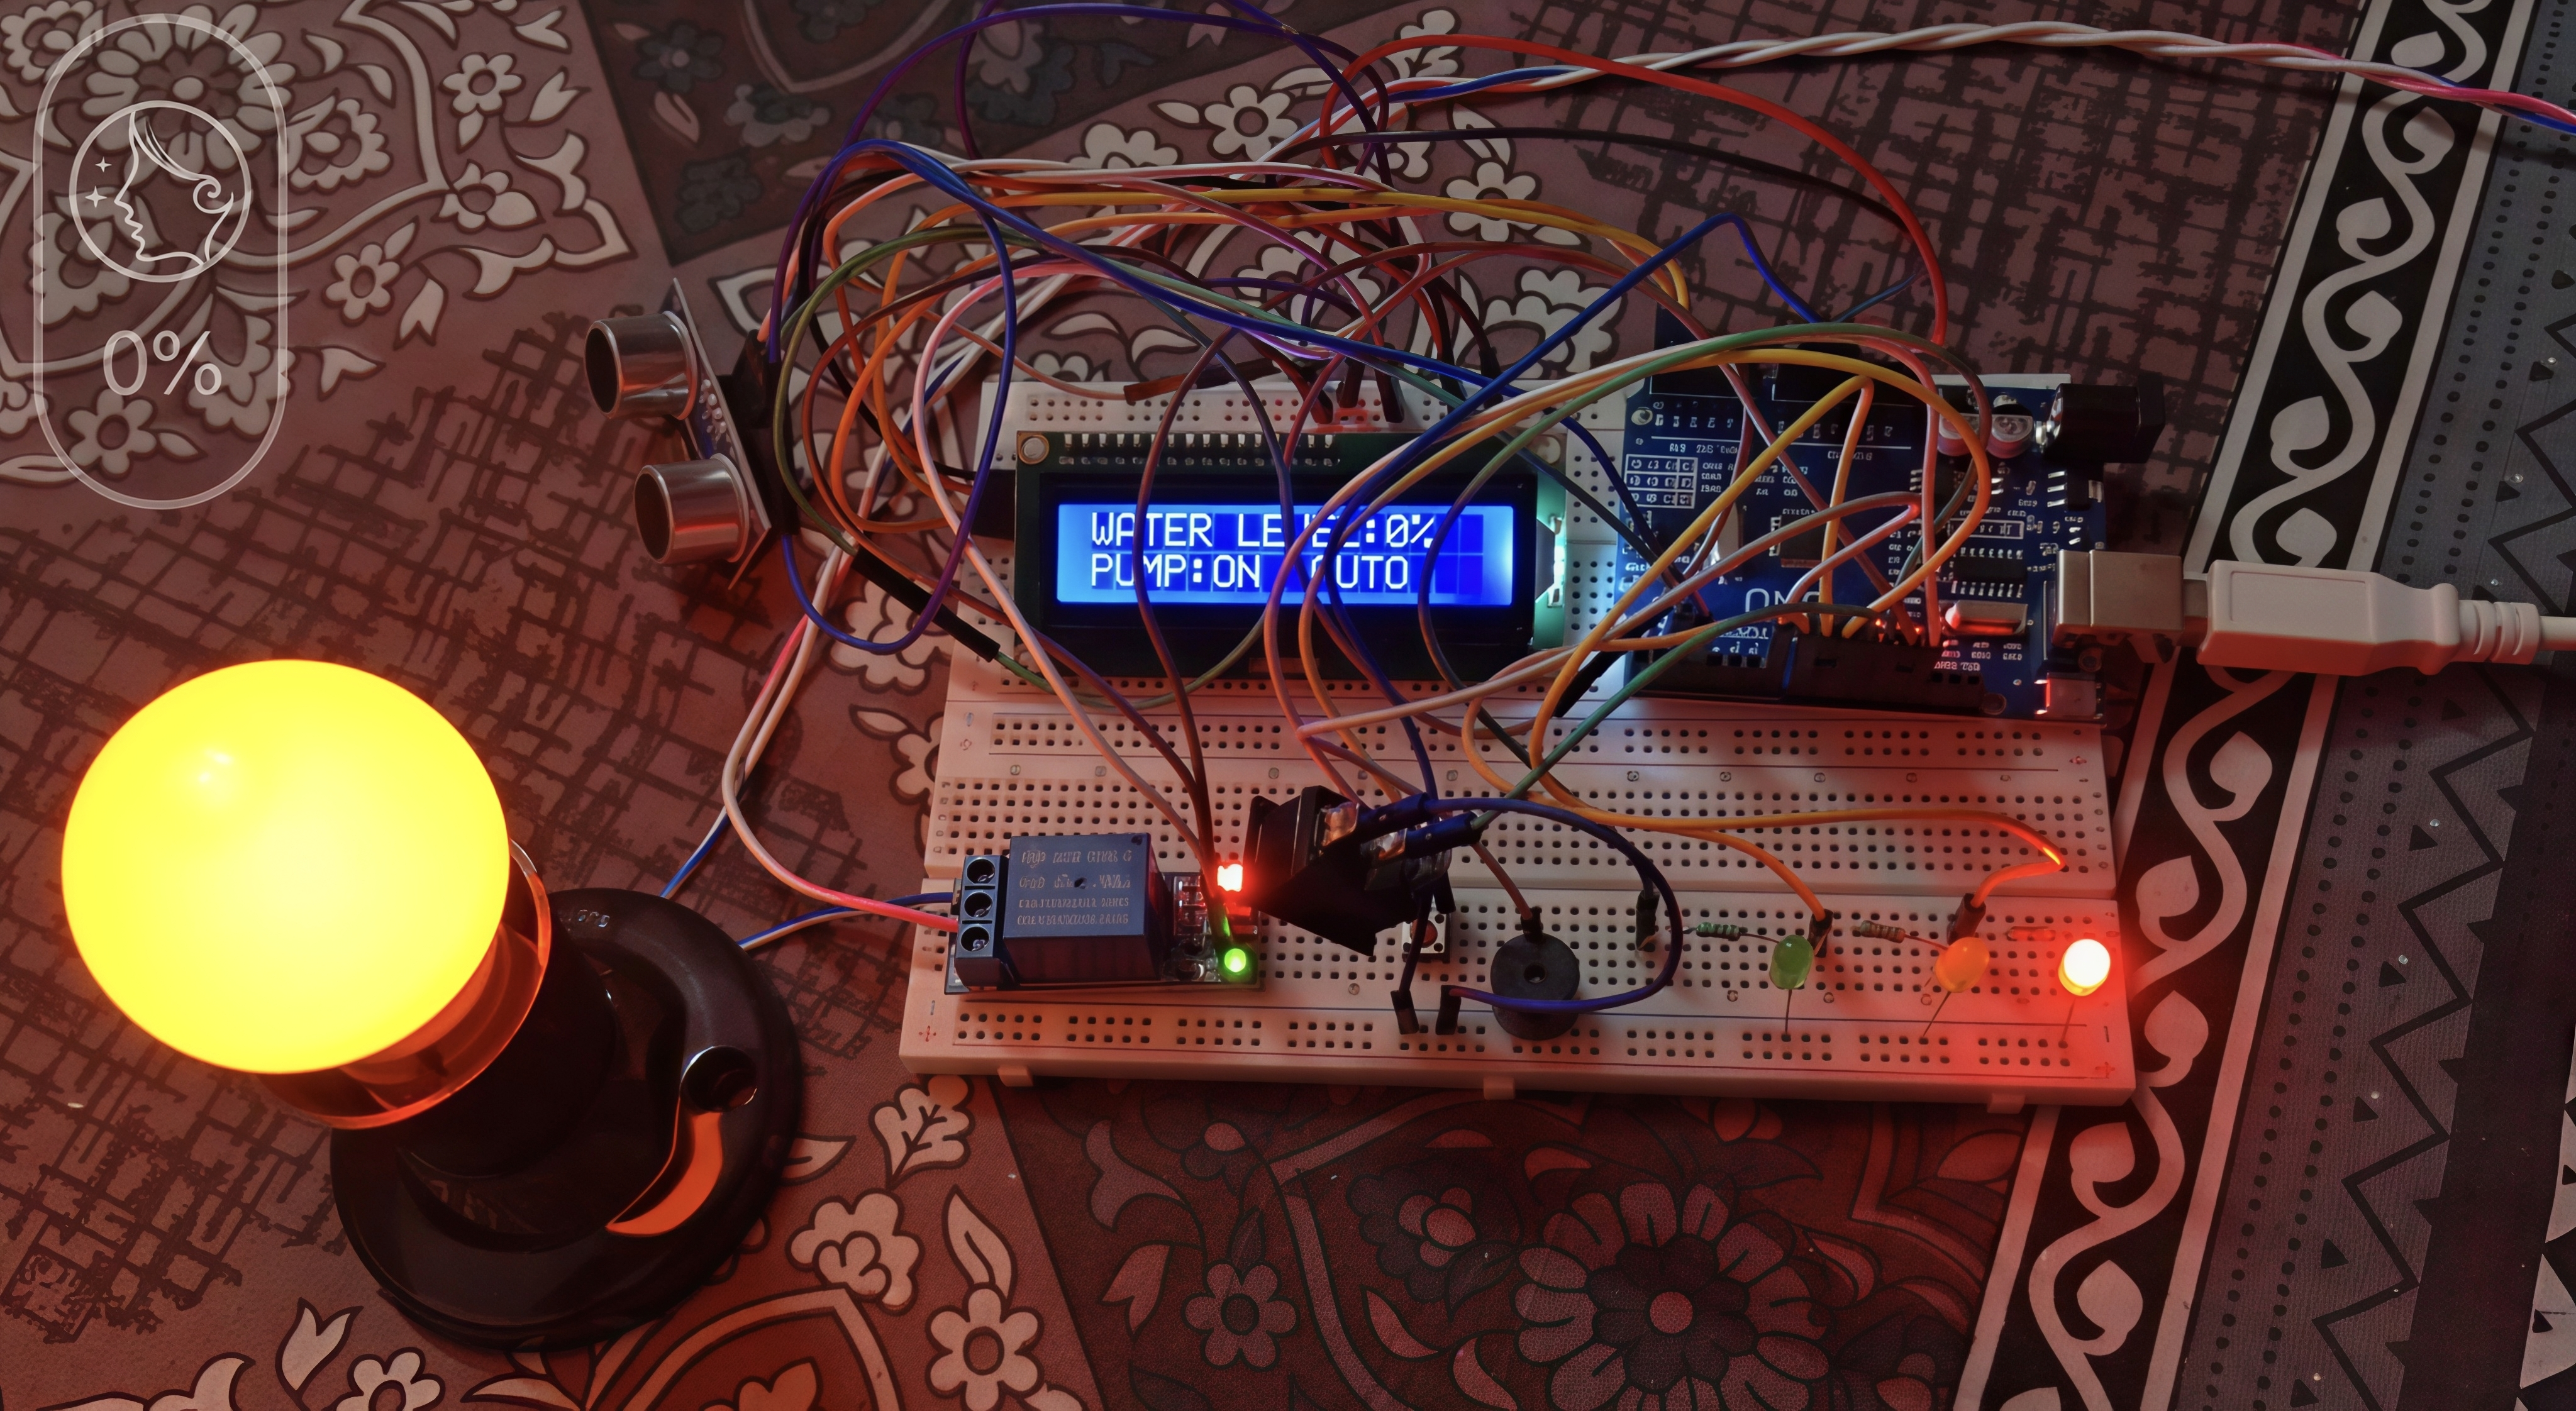
\includegraphics[width=0.82\textwidth]{../assets/hardware-setup.jpg}
\caption{Hardware Implementation of the Smart Water Tank Control System}
\label{fig:hardware}
\end{figure}

\section{SYSTEM TESTING}

The prototype was tested under different operating conditions.

\begin{table}[H]
\centering
\begin{tabular}{|p{5cm}|p{7cm}|}
\hline
Test Case & Result\\
\hline
Tank Empty & Pump turned ON automatically.\\
Tank Full & Pump turned OFF automatically.\\
Manual Mode & Pump toggled using push button.\\
AUTO Switch & Mode changed successfully.\\
LED Indicators & Correctly indicated water level.\\
Buzzer Alert & Activated at low water level.\\
CSV Logging & Live data stored successfully.\\
Dashboard & Real-time updates received.\\
\hline
\end{tabular}
\caption{System Validation}
\label{tab:validation}
\end{table}

\section{CONCLUSION}

The Smart Home Water Tank Monitoring and Automatic Control System provides an efficient and reliable approach to monitoring and managing household water levels. The system integrates an Arduino Uno, ultrasonic sensor, LCD display, relay module, LEDs, buzzer, and water pump to continuously monitor the tank level and automatically control the pumping operation according to predefined water-level conditions.

The automatic control mechanism helps prevent water overflow and reduces the need for continuous manual monitoring. The use of visual and audio indicators provides clear information about important tank conditions, while the LCD displays the current system status to the user. The system also incorporates protection against unsuitable pump operation, thereby improving the overall reliability of the setup.

In addition to real-time monitoring and automatic control, the project includes data logging and statistical analysis using Python and Excel. The collected information can be used to study water consumption, pump operating patterns, refill frequency, and potential water-wastage trends. This combination of automation and data analysis makes the system useful not only for controlling the water tank but also for understanding and improving water usage.

Overall, the project demonstrates how embedded systems, sensor interfacing, electrical control, and statistical analysis can be combined to develop a practical smart-home application. The proposed system provides a low-cost foundation for automated water management and can be further enhanced in the future by incorporating remote monitoring, wireless connectivity, multiple-tank support, and more advanced data analysis techniques.
\section{FUTURE SCOPE}
While the current Smart Home Water Tank Monitoring and Automatic Control System successfully demonstrates automated water level regulation, pump control, and statistical analysis, there are numerous avenues for enhancement and expansion. These improvements can elevate the system from a standalone solution to a fully integrated, intelligent, and scalable water management ecosystem. \\
\begin{itemize}
     

\item IoT integration with ESP8266/ESP32 for remote monitoring and control via smartphone

\item Push notifications and SMS alerts for critical tank conditions

\item Mobile application development for real-time data visualization and system control

\item Multi-tank support for larger residential and commercial buildings

\item Integration of flow sensors for volume-based consumption tracking

\item Integration of pressure sensors for leak detection

\item Integration of water quality sensors (pH, TDS, turbidity)

\item Machine learning for consumption prediction and anomaly detection

\item Predictive maintenance alerts for pump failures

\item Solar power integration for energy independence

\item Cloud data storage for long-term trend analysis

\item Voice control integration with Amazon Alexa / Google Home

\item Automated billing system for apartment complexes

\item Compact PCB design for commercialization

\item Integration with smart irrigation systems

\end{itemize}

\newpage

% ============================================================
% PROJECT REPOSITORY
% ============================================================



\section{REFERENCES}

[1] R. Wahyuni, J. T. Sentana, M. Muhardi, and Y. Irawan, ``Water Level Control Monitoring Based on Arduino Uno R3 Atmega328P Using LM016L LCD,'' Journal of Robotics and Control, vol. 2, no. 4, pp. 265--272, 2021.

[2] A. Amin, ``Monitoring Water Level Control Based on Arduino Uno Using LCD,'' EEICT Journal, vol. 1, no. 1, 2018.

[3] H. Zhang, W. Tao, and M. Cao, ``Development and Application of Mobile Water Level Monitoring Based on Multi-Sensor Integration,'' in Proc. Int. Conf. Electrical and Control Engineering, Wuhan, China, 2010.

[4] X. Cui, Z. Kou, and Y. Qiao, ``Water-Level Control System for Solar Water Heating Engineering Based on PLC,'' in 2019 IEEE 3rd Information Technology, Networking, Electronic and Automation Control Conference (ITNEC), Chengdu, China, 2019.

[5] ``Ultrasonic Water Level Indicator and Controller Using AVR Microcontroller,'' IEEE Conference Publication, 2017.

[6] ``Non-contact Water Level Monitoring System Implemented Using LabVIEW and Arduino,'' IEEE Conference Publication, 2017.

[7] V. K. S. Varun, K. A. Kumar, V. R. Chowdary, and C. Raju, ``Water Level Management Using Ultrasonic Sensor (Automation),'' International Journal of Computer Sciences and Engineering, vol. 6, no. 6, pp. 799--804, 2018.

[8] ``Embedded System Based Solution for Water Level Monitoring and Conservation,'' International Journal of Advanced Research, vol. 13, no. 11, pp. 19--25, 2025.

\end{document}